\documentclass[11pt,a4paper]{article}

\usepackage[margin=1in]{geometry}
\usepackage{amsmath,amssymb}
\usepackage{graphicx}
\usepackage{booktabs}
\usepackage{xcolor}
\usepackage{caption}
\usepackage{microtype}

\captionsetup{font=small,labelfont={bf},labelsep=period}
\usepackage[colorlinks=true,linkcolor=red!60!black,citecolor=green!45!black,urlcolor=blue!60!black]{hyperref}

\newcommand{\dex}{\ensuremath{\,\mathrm{dex}}}
\newcommand{\Khalf}{\ensuremath{K_{1/2}}}

\title{\textbf{Amplitude and midpoint statistics of the same chemotaxis cells\\ demand incompatible receptor models}}
\author{Huan Li\\[2pt]
\small Shanghai Liangta Biotech Co., Ltd., Shanghai 201899, China\\
\small Correspondence: hl@liangtabio.com\quad ORCID: 0009-0004-2695-6825}
\date{}

\begin{document}
\maketitle

\begin{abstract}
\noindent
The bacterial chemotaxis receptor layer is the most thoroughly modelled sensory system in biology, and the Monod--Wyman--Changeux (MWC) cluster model with perfect methylation-based adaptation is its standard description. Here we show that this model class fails a controlled joint test on the single-cell FRET dose-response archive of Moore \emph{et al.} (seven MeAsp backgrounds $0$--$100\,\mu$M, 57--268 cells per background). From the same raw trajectories we construct two statistics: the population amplitude table $R(B,F)$ and the per-cell midpoint distribution $\Khalf(B)$. The midpoints obey a Weber line, $\Khalf = 1.17\,(1.95+B)\,\mu$M, to within $0.10\dex$ across four decades of background, and its slope implies a receptor-cluster cooperativity of $N\approx2$--$4$; the amplitude table requires $N\approx12$--$39$. A Pareto scan of joint fits confirms that no parameter set of the standard class meets a pre-specified acceptance region (amplitude $R^2>0.9$, midpoint error $<0.1\dex$, physical saturation amplitude): the front's endpoints read $R^2=0.980$ with midpoint error $0.622\dex$ and $R^2=0.511$ with error $0.074\dex$. Eight minimal repair hypotheses, from subpopulations to asymmetric cooperativity, all fail the same criterion, and a same-source reconstruction restricted to non-censored cells leaves the rupture unmoved, excluding population-averaging artefacts. The empirical response kernel $R = 0.2268\,\ln(1+F/0.570)\,/\,(1+(B/69.7)^{0.778})$ ($R^2=0.967$) predicts the midpoints of two unseen mixed-ligand arms, frozen before data access, to within $+0.014$, $+0.038$ and $+0.031\dex$ at backgrounds outside the fitting domain. The rupture is therefore real, localised to the model's structural core, and compatible with passive MWC cluster-state equilibrium but not with active methylation-dependent retuning; a cheR/cheB fixed-methylation mutant experiment is proposed as the decisive test.
\end{abstract}

\section{Introduction}

\emph{Escherichia coli} chemotaxis couples ligand binding at receptor clusters to flagellar motor output through a short, well-mapped signalling pathway. Quantitatively, the receptor layer is described by two-state MWC models of receptor clusters \cite{Monod1965,SourjikBerg2002}, combined with methylation-based feedback that restores the adapted activity after a step change in ligand concentration \cite{BarkaiLeibler1997}. This framework explains adaptation exactness \cite{BarkaiLeibler1997}, response rescaling across backgrounds \cite{Lazova2011}, and the input-output relation measured by in vivo FRET \cite{SourjikBerg2002,Shimizu2010,Tu2008}.

A question that has not been settled is whether one parameter set of this standard class can generate the full dose-response structure of the receptor layer: not only how large the response is, but where, along the concentration axis, each cell's response sits. The single-cell archive of Moore \emph{et al.} \cite{Moore2024} makes this question decidable. It records FRET responses of individual cells to foreground concentration steps $F$ delivered on seven adaptation backgrounds $B$ spanning four decades ($0$ to $100\,\mu$M MeAsp), with 57 to 268 cells per background. Because the data are single-cell, two statistics can be built from the same trajectories: the population amplitude table $R(B,F)$, and the distribution of per-cell midpoints $\Khalf(B)$, the foreground concentration at which each cell reaches half of its own maximal response.

These two statistics constrain different parts of the model. The amplitude table measures response magnitudes; the midpoint distribution measures the concentration axis itself. We show that the standard model class cannot satisfy both at once, that the failure survives eight minimal repair hypotheses and a reconstruction designed to exclude censoring artefacts, and that an empirical response kernel fitted to the ruptured statistics nevertheless predicts unseen mixed-ligand arms with deviations of at most $0.04\dex$. The standard picture of the chemotaxis receptor layer is incomplete in a specific, measurable, and experimentally decidable way.

\section{Two statistics from the same cells}
\label{sec:statistics}

The Moore \emph{et al.} archive \cite{Moore2024} (Dryad doi:10.5061/dryad.nvx0k6dzz, CC0) contains single-cell FRET trajectories for foreground steps at five levels per background, across backgrounds $B=0,\,0.01,\,0.1,\,0.3,\,1,\,10,\,100\,\mu$M MeAsp.

\paragraph{Amplitude table.} Per condition, the population median of the plateau response gives the 30-row amplitude table $R(B,F)$.

\paragraph{Per-cell midpoints.} For each cell, the foreground concentration at half-maximal response, interpolated on the log-concentration axis, defines $\Khalf$. Cells whose maximal observed response is below $0.5$ are right-censored; 45--68\% of cells per background are censored (Fig.~\ref{fig:main}d), and we return to the consequences below. Per-background medians are $2.03$, $2.90$, $2.17$, $2.58$, $3.49$, $13.92$ and $119.56\,\mu$M for the seven backgrounds.

\paragraph{The Weber line.} The measured midpoints obey
\begin{equation}
\Khalf(B) = 1.17\,(1.95 + B)\ \mu\mathrm{M},
\label{eq:weber}
\end{equation}
with maximum deviation $0.10\dex$ and mean deviation $0.03\dex$ across four decades of background (Fig.~\ref{fig:main}c); the $B=10$ point lies on the line at $-0.002\dex$. A linear midpoint-versus-background law with slope near unity is the classical Weber behaviour of a sensory system whose detection threshold scales with the adapted level.

\section{The standard model class and the joint-fit test}
\label{sec:model}

\subsection{Model class}

A homogeneous cluster of $N$ allosterically coupled receptors in two activity states has activity
\begin{equation}
a(L) \;=\; \frac{(1+L/K_A)^{N}}{(1+L/K_A)^{N} + e^{\varepsilon}\,(1+L/K_I)^{N}},
\label{eq:mwc}
\end{equation}
with inactive-state and active-state dissociation constants $K_I < K_A$ and free-energy bias $\varepsilon$. Perfect adaptation retunes $\varepsilon$ through methylation so that the adapted activity returns to its ligand-independent set point \cite{BarkaiLeibler1997}; the measured step response on background $B$ is the activity increment from the adapted state,
\begin{equation}
R(B,F) = a_{\max}\,\big[\,a(B+F) - a_{\mathrm{adapted}}(B)\,\big],
\label{eq:response}
\end{equation}
and the model midpoint $\Khalf^{\mathrm{model}}(B)$ is defined implicitly by $R(B,\Khalf^{\mathrm{model}}) = \tfrac12 R(B,\infty)$.

\subsection{The cooperativity contradiction, in one line}

Within this class, the Weber slope of Eq.~\eqref{eq:weber} is tied to cooperativity: inverting the slope requires $N \approx 2$--$4$. The amplitude table, whose steepness grows with $N$, requires $N \approx 12$--$39$. The midpoint statistic sees a shallower dose-response than the amplitude statistic, and no single $N$ can serve both.

\subsection{Joint-fit protocol}

To make the contradiction precise we scanned joint fits of Eq.~\eqref{eq:response} to the amplitude table and the midpoint distribution along a Pareto front, varying the weight $\lambda$ between the amplitude $R^2$ objective and the midpoint absolute-error objective (in dex). The acceptance region, fixed before scoring, requires
\begin{equation}
R^2_{\mathrm{amplitude}} > 0.9,
\qquad
|\Delta \Khalf|_{\mathrm{mean}} < 0.1\dex,
\qquad
a_{\max} \approx 1 .
\label{eq:acceptance}
\end{equation}
The third condition is physical: the response amplitude is a normalised FRET increment and saturates near unity; fitted values of $1.4$--$2.8$ mark model strain.

\section{Results}

\subsection{The rupture: no point of the Pareto front is acceptable}
\label{sec:rupture}

The two endpoints of the front bracket the impossibility (Fig.~\ref{fig:main}a). At $\lambda=0$ (amplitude only), the fit reaches $R^2 = 0.980$ but the midpoint error is $0.622\dex$, with parameters $K_I = 30.7$, $K_A = 133\,\mu$M, $N = 39$, $a_{\max} = 1.39$. At $\lambda=30$ (midpoint-priority), the midpoint error falls to $0.074\dex$ but the amplitude fit collapses to $R^2 = 0.511$ ($K_I = 4.3\,\mu$M, $N = 2.0$). No intermediate weight enters the acceptance region \eqref{eq:acceptance}. The fitted $a_{\max}$ exceeds its physical value wherever the amplitude is fit well. The standard model class, as a single-parameter-set description of this dataset, is ruptured.

\begin{figure}[p]
\centering
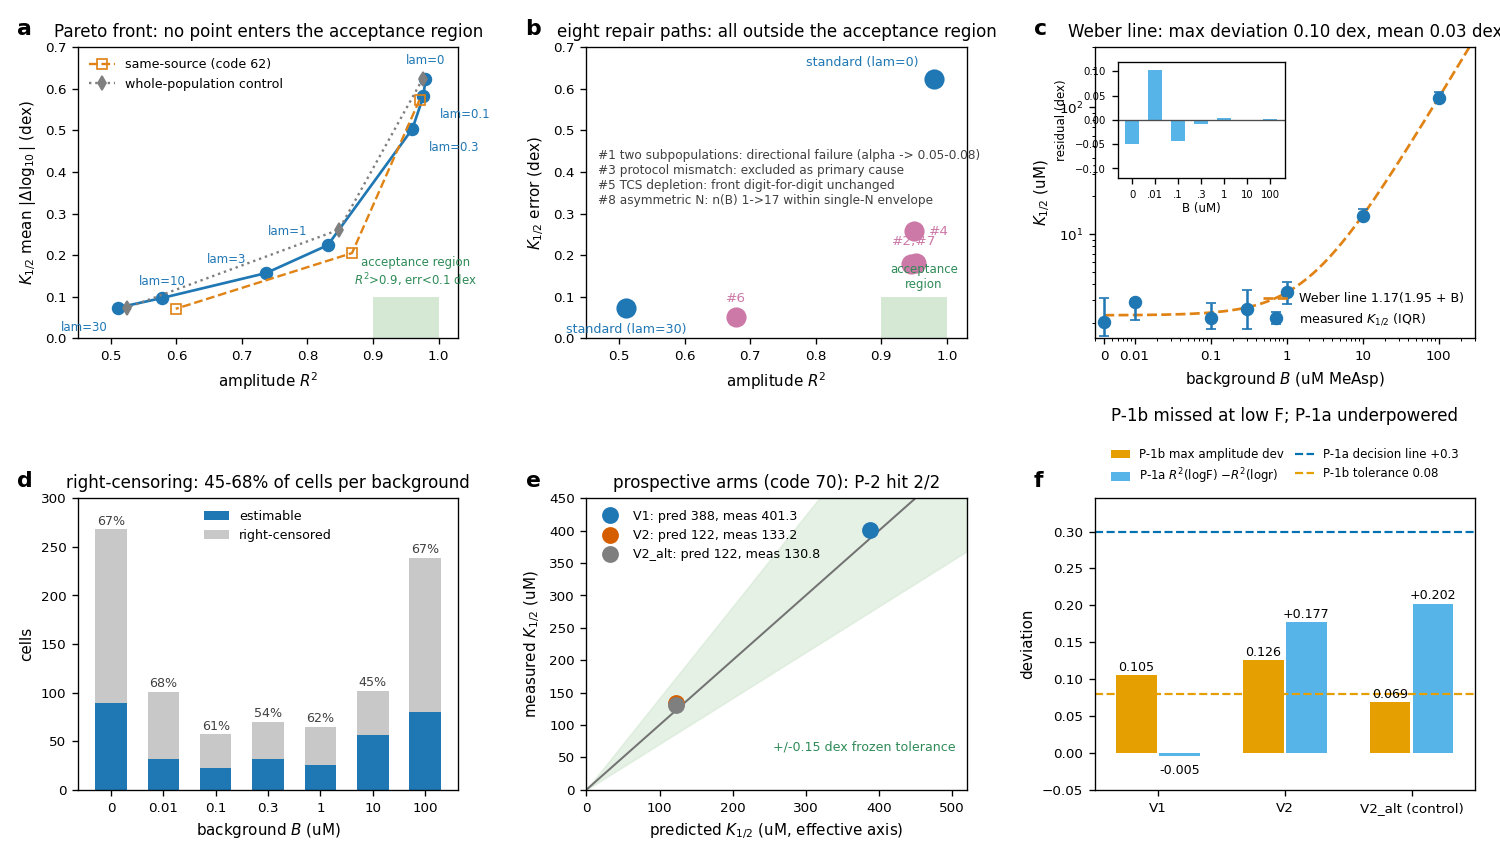
\includegraphics[width=\textwidth]{fig1_chemotaxis.png}
\caption{The chemotaxis receptor-layer rupture and its prospective test. \textbf{a}, Pareto front of joint fits (amplitude $R^2$ versus midpoint error), for the whole-population construction and the same-source construction restricted to non-censored cells; the shaded box marks the acceptance region, which no point enters. \textbf{b}, Eight minimal repair hypotheses scored in the same coordinates; the four returning a single best-fit point are plotted (\#2, \#4, \#6 and \#7, with \#2 and \#7 near-coincident) and the rest are annotated with their rejection reasons; none enters the acceptance region. \textbf{c}, The Weber line of measured per-cell midpoints (Eq.~\eqref{eq:weber}); inset, residuals in dex. \textbf{d}, Right-censoring fraction per background (45--68\%). \textbf{e}, Prospective mixed-ligand arms: predicted versus measured midpoints for arms V1, V2 and the ambiguity control V2\_alt, with the frozen $\pm0.15\dex$ tolerance band. \textbf{f}, Amplitude and structural clauses of the prospective test: maximum amplitude deviations (orange, tolerance $0.08$) and structural discrimination scores (blue, decision line $+0.3$).}
\label{fig:main}
\end{figure}

\subsection{Eight minimal repairs all fail}
\label{sec:repairs}

Each row of Table~\ref{tab:repairs} is a minimal extension or perturbation of the standard model, scored against the same acceptance criterion. The failures are informative. Two-subpopulation mixtures fail directionally, with the mixture weight driven to $0.05$--$0.08$; imperfect adaptation improves the fit only by driving $K_A\to\infty$; gain retuning meets the midpoint statistic ($0.052\dex$) only by abandoning the amplitude table ($R^2 = 0.68$) at non-physical parameter bounds; population heterogeneity is rejected by the optimizer itself, which shrinks the spread parameter in the direction opposite to the hypothesis; and asymmetric cooperativity is excluded because the measured apparent Hill coefficient, rising from $\sim$1 to 17 across backgrounds, lies everywhere within the envelope of single-$N$ MWC controls, so no steepness beyond one cooperativity exists in the data. Ligand depletion, though formally present (depletion ratio $\kappa \approx 48$), leaves the Pareto front digit-for-digit unchanged once the implicit free-ligand equation is solved.

\begin{table}[!htbp]
\centering
\caption{Eight minimal repair hypotheses, scored under the acceptance region of Eq.~\eqref{eq:acceptance}.}
\label{tab:repairs}
\small
\begin{tabular}{@{}clp{5.6cm}@{}}
\toprule
\# & Hypothesis & Best result; reason rejected \\
\midrule
1 & Two subpopulations (fast-adapting + non-adapting) & Directional failure; mixture weight driven to $0.05$--$0.08$, worse than single-species fit \\
2 & Imperfect adaptation ($\beta<1$) & Best $R^2=0.953$ / $0.182\dex$; improvement comes from $K_A\to\infty$, not from $\beta$ \\
3 & Protocol mismatch (step vs.\ waveform pre-adaptation) & Step responses are $\log F$-dominated; excluded as primary cause \\
4 & FRET readout nonlinearity (three variants) & Best $R^2=0.950$ / $0.257\dex$; excluded as sole cause \\
5 & Ligand depletion ($\kappa\approx48$) & Front digit-for-digit unchanged after solving free-ligand equation \\
6 & Background-dependent gain retuning & Midpoint side $0.052\dex$ but amplitude $R^2$ collapses to $0.68$; non-physical bounds \\
7 & Population heterogeneity + censoring & Best $0.946$ / $0.179\dex$; optimizer shrinks spread opposite to hypothesis \\
8 & Asymmetric cooperativity ($N_T\approx2$--$4$, $N_R\approx12$--$39$) & Measured apparent $n(B)$ within single-$N$ envelope; two $N$ values not required \\
\bottomrule
\end{tabular}
\end{table}

\subsection{The rupture is not a censoring artefact}
\label{sec:samesource}

Because 45--68\% of cells are right-censored, the midpoint median is a sensitive-subpopulation statistic while the amplitude table is a whole-population median, and one might suspect the rupture is manufactured by comparing different cell ensembles. The single-cell archive allows a direct control: rebuild the amplitude table from strictly the same non-censored cells (32--55\% per background) that yield estimable midpoints, and re-run the joint fit. The Pareto front does not move (Table~\ref{tab:samesource}). The rupture persists inside a strictly single population; it is not a statistic-sampling artefact.

\begin{table}[!htbp]
\centering
\caption{Same-source control: joint fits rebuilt from non-censored cells only, versus whole-population.}
\label{tab:samesource}
\small
\begin{tabular}{@{}lll@{}}
\toprule
$\lambda$ & Same-source (sensitive subpopulation) & Whole-population control \\
\midrule
0  & $R^2=0.971$ / $0.573\dex$ & $R^2=0.976$ / $0.624\dex$ \\
1  & $R^2=0.868$ / $0.205\dex$ & $R^2=0.848$ / $0.261\dex$ \\
30 & $R^2=0.599$ / $0.071\dex$ & $R^2=0.525$ / $0.074\dex$ \\
\bottomrule
\end{tabular}
\end{table}

\subsection{An empirical kernel that works, and a naive kernel that does not}
\label{sec:kernel}

The ruptured statistics are themselves highly structured. The amplitude table is described by a four-parameter empirical kernel,
\begin{equation}
R(F,B) \;=\; A\,\frac{\ln\!\big(1 + F/K_c\big)}{1 + (B/B_s)^{p}},
\qquad
A = 0.2268,\; K_c = 0.570\,\mu\mathrm{M},\; B_s = 69.7\,\mu\mathrm{M},\; p = 0.778,
\label{eq:g10}
\end{equation}
with $R^2 = 0.967$ on the 30-row table. Two features matter. The numerator is an absolute increment, $\ln(1+F/K_c)$, anchored at a structural constant $K_c$ rather than at the background; and the denominator supplies the background suppression. By contrast, the naive MWC occupancy-increment kernel $\theta(L) = L/(K_d + L)$ predicts a multiplicative response structure that the data flatly reject: it achieves $R^2(\log F) = 0.000$ against the empirical $0.652$, predicting a response of $0.003$ where $0.424$ is measured at $B=100$, $F=40\,\mu$M. Occupancy increment is not the receptor layer's response kernel.

\subsection{Prospective validation on unseen mixed-ligand arms}
\label{sec:prospective}

The kernel's worth is decided on data it has never seen. Predictions for two mixed-ligand arms were frozen on 2026-08-16, before the corresponding files were downloaded. The frozen inputs were Eq.~\eqref{eq:g10}, the cross-ligand potency ratio $\rho = 23$ ($1\,\mu$M L-Asp equivalent to $23\,\mu$M MeAsp, so $B_{\mathrm{eff}} = B_{\mathrm{MeAsp}} + 23\,B_{\mathrm{L\text{-}Asp}}$), and the Weber line \eqref{eq:weber}. Both arms lie outside the fitting domain ($B \le 100\,\mu$M), so these are extrapolations.

The midpoint clauses all hit (Fig.~\ref{fig:main}e; tolerance $\pm0.15\dex$): arm V1 ($B_{\mathrm{eff}}=330\,\mu$M, 120 cells), predicted $388\,\mu$M, measured median $401.3\,\mu$M (IQR 388.5--407.6), deviation $+0.014\dex$, with the predicted high censoring observed (82\%); arm V2 ($B_{\mathrm{eff}}=102.3\,\mu$M, 156 cells), predicted $122\,\mu$M, measured $133.2\,\mu$M (IQR 122.8--140.4), $+0.038\dex$; the ambiguity control V2\_alt, measured $130.8\,\mu$M, $+0.031\dex$. The foreground-axis point prediction, $0.86\,\mu$M L-Asp, came out against measured values of $1.24$--$1.34\,\mu$M.

The amplitude clauses missed in the kernel's known weak region (Fig.~\ref{fig:main}f): maximum deviations $0.105$ (V1) and $0.126$ (V2) against a tolerance of $0.08$, with the miss concentrated at low $F$ and convergence at high $F$, reproducing the shortfall previously recorded in the same-source arms. The structural clause (a discrimination score with decision line $+0.3$) was missed in all readings ($-0.005$, $+0.177$, $+0.202$); in the $B_{\mathrm{eff}}=330$, $F\le80$ window the two coordinates being discriminated are compressed into a $0.007$--$0.094$ range and are mathematically near-degenerate, so the line is physically unreachable in this regime, a limitation of the test design rather than of the kernel.

The net account: the concentration axis of unseen mixed-ligand arms is predicted to within $0.04\dex$ by a four-parameter kernel frozen in advance, while the amplitude at low foreground carries a registered, repeatable shortfall.

\subsection{Mechanism: one candidate excluded, one standing}
\label{sec:mechanism}

Two candidate mechanisms for the rupture's steepness source were tested against the archived evidence. Candidate (a), active methylation-state-dependent retuning of receptor-cluster effective parameters, is excluded twice over: by repair path 6, which reaches the midpoint statistic only by collapsing the amplitude fit at non-physical parameter bounds, and by the cross-ligand arm, where a constant potency ratio $\rho \approx 22$--$24$ with pure competitive MWC occupancy suffices (residual $-0.045\dex$ at $F=5\,\mu$M), leaving no room for ligand-specific retuning. Candidate (b), passive MWC cluster-state equilibrium, is qualitatively compatible (the measured apparent Hill curve lies within the single-$N$ envelope throughout) but quantitatively non-closing. The rupture therefore stands, and the decisive experiment is a cheR/cheB fixed-methylation mutant pair measured on both statistics: if the rupture survives fixed methylation, candidate (b) is confirmed as structural; if it collapses, methylation dynamics re-enters through a mechanism outside the minimal form of (a).

\section{Discussion}

The chemotaxis receptor layer is usually presented as a solved system. The result here is narrower and more useful than a general challenge: within the standard model class, the concentration axis (where cells respond) and the amplitude axis (how much they respond) cannot be generated by one parameter set, and the failure is quantified, $0.62\dex$ of midpoint error at the amplitude-optimal fit, or a collapsed amplitude fit at the midpoint-optimal point. Because the same-source control leaves the front unmoved, the discrepancy is a structural property of the model class, not of the statistics.

The empirical kernel \eqref{eq:g10} deserves attention in its own right. Its numerator is an absolute log-increment anchored at $K_c = 0.57\,\mu$M, not a fold change in total ligand; its prospective extrapolation to mixed-ligand backgrounds nearly four-fold beyond the fitting domain lands within $0.04\dex$ on the midpoint axis. Whatever the correct structural model is, it must reproduce this functional form. The registered low-$F$ amplitude shortfall marks where the kernel, too, is incomplete.

For the fold-change-detection debate, the structural clause carries a methodological lesson: in regimes where the ratio coordinate is compressed (here $0.007$--$0.094$), discrimination between increment-based and ratio-based readouts is physically unreachable, and reported preferences between the two should be quoted with the coordinate range in which they were measured.

The limitations are explicit. The analysis rests on one archive, albeit the most complete single-cell dose-response archive available. Right-censoring is substantial at extreme backgrounds, and although the same-source control closes the population-averaging objection, midpoint medians remain sensitive-subpopulation statistics. The midpoint-versus-amplitude conflict is demonstrated for the standard MWC-plus-perfect-adaptation class; models outside this class are not excluded. Finally, the decisive cheR/cheB mutant experiment is proposed, not performed.

\section{Methods}
\label{sec:methods}

\subsection{Data and statistics construction}

The archive of Moore \emph{et al.} \cite{Moore2024} (Dryad doi:10.5061/dryad.nvx0k6dzz, CC0) was used as released. Plateau responses were extracted per cell and condition; the amplitude table $R(B,F)$ collects population medians across the 30 background-by-foreground units. Per-cell midpoints $\Khalf$ were interpolated on the log-concentration axis at half of each cell's maximal observed response; cells with maximal response below $0.5$ were right-censored. Censoring fractions are reported per background in Fig.~\ref{fig:main}d.

\subsection{Model fitting and the Pareto protocol}

The model class of Section~\ref{sec:model} was fit jointly to the amplitude table (least squares, reported as $R^2$) and the per-background midpoint medians (absolute error in dex), with the weight $\lambda$ between the two objectives swept to trace the Pareto front. The acceptance region \eqref{eq:acceptance} was fixed before scoring. Multi-start optimization was used throughout; an early implementation with infeasible parameter bounds was caught by infeasibility of all starts and corrected.

\subsection{Repair-path implementations}

Each hypothesis of Table~\ref{tab:repairs} was implemented as the minimal modification of the standard model expressing it: mixture weight for subpopulations; a $\beta<1$ adaptation factor; protocol-shape-stratified re-analysis; power-law FRET readout remaps; the implicit free-ligand equation for depletion with $\kappa\approx48$; per-background effective parameters for gain retuning; a free population-spread parameter for heterogeneity; and per-row apparent Hill coefficients against single-$N$ MWC controls for asymmetric cooperativity.

\subsection{Same-source control}

The amplitude table was rebuilt using only cells with estimable midpoints (32--55\% per background), and the joint fit re-run under the identical protocol (Table~\ref{tab:samesource}).

\subsection{Prospective arm freezing and scoring}

Prediction inputs (Eq.~\eqref{eq:g10}, $\rho=23$, Weber line) were frozen in writing on 2026-08-16 before the mixed-ligand files (arms of 2023-08-22/23 and 2023-10-17/18 in the archive) were downloaded. File identity was verified against the archive's condition list using the recorded stimulus fields before scoring; one extraction-convention error on our side (arm V1's stimulus field records total MeAsp because foreground and background are the same ligand) was caught by this check and corrected before scoring. Tolerances were frozen with the predictions ($\pm0.15\dex$ midpoints; $0.08$ amplitude; $+0.3$ structural line).

\subsection{Quality control}

Three internal pipeline errors were caught and repaired during the analysis, each verified by an independent rerun: a parameter-unpacking order error, a foreground-versus-total concentration convention error (corrected as $F = s_v - B$), and the infeasible-bounds error above. No result changed after repair.

\subsection{Reproducibility}

Every number in the text regenerates from named analysis scripts (codes 51--62 and 70) run against the archived tables, available at github.com/lihuanlz/chemotaxis-receptor-layer, archived at Zenodo (doi:10.5281/zenodo.23402856; umbrella edition: doi:10.5281/zenodo.23008824).

\section*{Data and code availability}

No new experimental data were generated. The Moore \emph{et al.} archive is public (Dryad doi:10.5061/dryad.nvx0k6dzz, CC0). All analysis scripts, extracted tables, frozen prediction documents and scoring outputs are available at github.com/lihuanlz/chemotaxis-receptor-layer, archived at Zenodo (doi:10.5281/zenodo.23402856; umbrella edition: doi:10.5281/zenodo.23008824).

\section*{Acknowledgements}

We thank J.~P.~Moore, K.~Kamino, T.~S.~Shimizu, T.~Emonet and colleagues for the chemotaxis FRET dose-response archive, released CC0 with foreground, background and mixed-ligand arms complete enough to support prospective blind tests.

\section*{Author contributions}

H.L.\ conceived the study, derived the tests, wrote and validated the analysis code, performed the analysis, and wrote the paper.

\section*{Competing interests}

The author declares no competing interests.

\begin{thebibliography}{99}
\small

\bibitem{Moore2024}
Moore, J.~P., Kamino, K., Kottou, R., Shimizu, T.~S. \& Emonet, T. Signal integration and adaptive sensory diversity tuning in \emph{Escherichia coli} chemotaxis. \emph{Cell Syst.} \textbf{15}, 628--638 (2024).

\bibitem{Monod1965}
Monod, J., Wyman, J. \& Changeux, J.-P. On the nature of allosteric transitions: a plausible model. \emph{J. Mol. Biol.} \textbf{12}, 88--118 (1965).

\bibitem{BarkaiLeibler1997}
Barkai, N. \& Leibler, S. Robustness in simple biochemical networks. \emph{Nature} \textbf{387}, 913--917 (1997).

\bibitem{SourjikBerg2002}
Sourjik, V. \& Berg, H.~C. Receptor sensitivity in bacterial chemotaxis. \emph{Proc. Natl Acad. Sci. USA} \textbf{99}, 123--127 (2002).

\bibitem{Shimizu2010}
Shimizu, T.~S., Tu, Y. \& Berg, H.~C. A modular gradient-sensing network for chemotaxis in \emph{Escherichia coli} revealed by responses to time-varying stimuli. \emph{Mol. Syst. Biol.} \textbf{6}, 382 (2010).

\bibitem{Tu2008}
Tu, Y., Shimizu, T.~S. \& Berg, H.~C. Modeling the chemotactic response of \emph{Escherichia coli} to time-varying stimuli. \emph{Proc. Natl Acad. Sci. USA} \textbf{105}, 14855--14860 (2008).

\bibitem{Lazova2011}
Lazova, M.~D., Ahmed, T., Bellomo, D., Stocker, R. \& Shimizu, T.~S. Response rescaling in bacterial chemotaxis. \emph{Proc. Natl Acad. Sci. USA} \textbf{108}, 13870--13875 (2011).

\end{thebibliography}

\end{document}
